\chapter{生物合成与整合的细胞}\label{ch:b1:biosyntheses-integration}

早上八点，肝脏正把早餐中的糖转化为
\omterm{def:b1:carbohydrates:polysaccharide}{糖原}和\omterm{def:b1:lipids:triglyceride}{脂肪}；次日凌晨三点，同一个肝脏
正把肌肉中的\omterm{def:b1:proteins:aminoacid}{氨基酸}转化为糖，并将其输入血液，
供给已经九个小时未进食的大脑。酶本身并无改变，
改变的是哪些酶处于开启状态。
前面各章拆解了\omterm{def:b1:cell-unit-of-life:cell}{细胞}中的分子，本章则
将它们重新组装——糖、\omterm{def:b1:carbohydrates:polysaccharide}{糖原}、\omterm{def:b1:lipids:triglyceride}{脂肪}和\omterm{def:b1:proteins:aminoacid}{氨基酸}的合成，
然后探讨\omterm{def:b1:cell-unit-of-life:cell}{细胞}和\omterm{def:b1:organism-environment:organism}{生物体}如何在每一时刻决定
哪些代谢途径运行。答案在于一小套共用的
通用“货币”、位于交汇点的少数几种酶，以及
向每个\omterm{def:b1:cell-unit-of-life:cell}{细胞}传递整体状态的激素。

\section{合成需要什么}

\begin{proposition}[合成代谢的三项需求]\label{prop:b1:biosyntheses-integration:needs}
\index{合成代谢}
每一个生物合成都需要\emph{碳骨架}，它们取自\omterm{def:b1:respiration-fermentation:glycolysis}{糖酵解}和\omterm{def:b1:respiration-fermentation:krebs}{克雷布斯循环}的
少数几种中间产物；还需要\emph{还原
力}，由 \omterm{def:b1:biosyntheses-integration:ppp}{NADPH} 提供；以及\emph{能量}，由 \omterm{def:b1:water-small-molecules:atp}{ATP} 提供。
因此，分解代谢与合成代谢在相同的交汇点相遇——
6-磷酸葡萄糖、磷酸丙糖、丙酮酸、乙酰\omterm{def:b1:enzymes:enzyme}{辅酶} A，
$\alpha$-酮戊二酸、草酰乙酸——但在不可逆步骤上由各自独立的酶催化，
从而两个方向可以独立地开启或关闭，
二者还使用各自的\omterm{def:b1:enzymes:enzyme}{辅酶}传递电子：
NADH 保持氧化态，用于分解代谢中夺取电子；\omterm{def:b1:biosyntheses-integration:ppp}{NADPH}
保持还原态，用于合成中提供电子。
\end{proposition}

\begin{definition}[戊糖磷酸途径]\label{def:b1:biosyntheses-integration:ppp}
\index{戊糖磷酸途径}\index{NADPH}
\omterm{def:b1:eukaryotic-cell:organelle}{细胞溶胶}中的\emph{戊糖磷酸途径}将
6-磷酸葡萄糖氧化为 5-磷酸核\omterm{def:b1:carbohydrates:monosaccharide}{酮糖}和 $\mathrm{CO_2}$，
同时将两个 $\mathrm{NADP^+}$ 还原为 NADPH；其非氧化分支随后
使五碳、四碳、六碳和七碳糖磷酸相互转化，
于是\omterm{def:b1:cell-unit-of-life:cell}{细胞}在需要戊糖时可生成用于合成\omterm{def:b1:nucleic-acids:nucleotide}{核苷酸}的 5-磷酸核糖，
在需要还原力（\omterm{def:b1:lipids:triglyceride}{脂肪}合成、抵御氧化剂）时生成 NADPH，
或两者兼有，并将其余部分送回\omterm{def:b1:respiration-fermentation:glycolysis}{糖酵解}。它是
动物\omterm{def:b1:cell-unit-of-life:cell}{细胞}中 NADPH 的主要来源；在植物中，白天则由\omterm{def:b1:photosynthesis:chloroplast}{叶绿体}的
\omterm{prop:b1:photosynthesis:lightreactions}{光反应}提供 NADPH。
\end{definition}

\begin{omfigure}
\begin{tikzpicture}[font=\footnotesize, >=Stealth, line cap=round,
  hub/.style={draw, thick, rounded corners=3pt, fill=omDef!12, inner sep=3pt, align=center},
  prod/.style={draw, thick, rounded corners=3pt, fill=omExo!15, inner sep=3pt, align=center},
  fuel/.style={draw, thick, rounded corners=3pt, fill=omProp!15, inner sep=3pt, align=center}]
  \node[hub] (g6p) at (0,4.5) {6-磷酸葡萄糖};
  \node[hub] (tp) at (0,2.8) {磷酸丙糖};
  \node[hub] (pyr) at (0,1.1) {丙酮酸};
  \node[hub] (accoa) at (0,-0.6) {乙酰辅酶 A};
  \node[hub] (krebs) at (0,-2.4) {克雷布斯循环 \\ ($\alpha$-KG, OAA)};
  \draw[<->, thick] (g6p) -- (tp); \draw[<->, thick] (tp) -- (pyr); \draw[->, thick] (pyr) -- (accoa); \draw[->, thick] (accoa) -- (krebs);
  % left: stores and fuels in
  \node[fuel] (gly) at (-4.2,4.5) {糖原、淀粉}; \draw[<->, thick] (gly) -- (g6p);
  \node[fuel] (lac) at (-4.2,1.1) {乳酸}; \draw[<->, thick] (lac) -- (pyr);
  \node[fuel] (fa) at (-4.2,-0.6) {脂肪酸}; \draw[<->, thick] (fa) -- (accoa) node[pos=0.62, below=2pt, font=\scriptsize] {$\beta$-氧化 / 合成};
  \node[fuel] (aa) at (-4.2,-2.4) {氨基酸}; \draw[<->, thick] (aa) -- (krebs) node[pos=0.4, below=2pt, font=\scriptsize] {转氨作用};
  % right: products
  \node[prod] (ppp) at (4.3,4.5) {戊糖磷酸途径：\\ NADPH、5-磷酸核糖 $\to$ 核苷酸}; \draw[->, thick] (g6p) -- (ppp);
  \node[prod] (glyc) at (4.3,2.8) {甘油 $\to$ 脂质}; \draw[->, thick] (tp) -- (glyc);
  \node[prod] (ala) at (4.3,1.1) {丙氨酸、丝氨酸、甘氨酸}; \draw[<->, thick] (pyr) -- (ala);
  \node[prod] (chol) at (4.3,-0.6) {胆固醇、类固醇；\\ 酮体}; \draw[->, thick] (accoa) -- (chol);
  \node[prod] (glu) at (4.3,-2.4) {谷氨酸、天冬氨酸 \\ 及其家族；血红素}; \draw[<->, thick] (krebs) -- (glu);
  \draw[->, very thick, omThm] (1.4,-2.0) -- (1.4,0.65) node[pos=0.5, rotate=90, anchor=south, font=\scriptsize, omThm] {糖异生};
\end{tikzpicture}

{\small 代谢的交汇点。中心途径的六个枢纽（蓝色）
接收燃料与储备（橙色），并为各类生物合成（绿色）提供原料。
\omterm{def:b1:biosyntheses-integration:gluconeogenesis}{糖异生}（红色）使图的中段自下而上运行。}
\end{omfigure}

\section{葡萄糖的合成：糖异生}

\begin{definition}[糖异生]\label{def:b1:biosyntheses-integration:gluconeogenesis}
\index{糖异生}
\emph{糖异生}以非\omterm{def:b1:carbohydrates:monosaccharide}{糖类}为前体合成葡萄糖，
——乳酸、丙酮酸、甘油及大多数\omterm{def:b1:proteins:aminoacid}{氨基酸}的
碳骨架——，主要在肝脏中进行（肾脏中也有少量）。
它反向经过\omterm{def:b1:respiration-fermentation:glycolysis}{糖酵解}的七个可逆步骤，
并以不同的酶绕过三个不可逆步骤：丙酮酸先羧化为
草酰乙酸（在\omterm{def:b1:eukaryotic-cell:mitochondrion}{线粒体}中消耗一个 \omterm{def:b1:water-small-molecules:atp}{ATP}），再脱羧为磷酸烯醇式丙酮酸
（消耗一个 GTP）；1,6-二磷酸果糖水解为6-磷酸果糖；
6-磷酸葡萄糖水解为游离葡萄糖，并离开\omterm{def:b1:cell-unit-of-life:cell}{细胞}。每分子葡萄糖
需 6 个 \omterm{def:b1:water-small-molecules:atp}{ATP} 当量和 2 个 NADH，而\omterm{def:b1:respiration-fermentation:glycolysis}{糖酵解}仅产生 2 个 \omterm{def:b1:water-small-molecules:atp}{ATP}——
这正是让下坡路径逆向运行所付出的
代价。
\end{definition}

\begin{omfigure}
\begin{tikzpicture}[font=\footnotesize, >=Stealth, line cap=round,
  m/.style={draw, thick, rounded corners=3pt, inner sep=3pt, fill=omDef!10, align=center}]
  \node[m] (glc) at (0,5.2) {葡萄糖};
  \node[m] (g6p) at (0,3.9) {6-磷酸葡萄糖};
  \node[m] (f6p) at (0,2.6) {6-磷酸果糖};
  \node[m] (fbp) at (0,1.3) {1,6-二磷酸果糖};
  \node[m] (pep) at (0,-0.5) {磷酸烯醇式丙酮酸};
  \node[m] (pyr) at (0,-1.9) {丙酮酸};
  \node[m] (oaa) at (5.2,-1.9) {草酰乙酸};
  % glycolysis (down, left side)
  \draw[->, thick, omDef!70!black] (glc.west) ++(-0.2,0) -- ++(-1.0,0) |- (g6p.west) node[pos=0.25, left, font=\scriptsize, align=right] {己糖激酶 \\ ATP};
  \draw[->, thick, omDef!70!black] (f6p.west) ++(-0.2,0) -- ++(-1.0,0) |- (fbp.west) node[pos=0.25, left, font=\scriptsize, align=right] {PFK\\ ATP};
  \draw[->, thick, omDef!70!black] (pep.west) ++(-0.2,0) -- ++(-1.0,0) |- (pyr.west) node[pos=0.25, left, font=\scriptsize, align=right] {丙酮酸激酶 \\ 生成 ATP};
  \draw[<->, thick] (g6p) -- (f6p); \draw[<->, thick] (fbp) -- (pep) node[midway, right, font=\scriptsize] {可逆步骤（共用）};
  % gluconeogenesis (up, right side)
  \draw[->, thick, omThm] (g6p.east) ++(0.2,0) -- ++(1.0,0) |- (glc.east) node[pos=0.25, right, font=\scriptsize, align=left] {葡萄糖-6-磷酸酶 \\ （仅肝脏）};
  \draw[->, thick, omThm] (fbp.east) ++(0.2,0) -- ++(1.0,0) |- (f6p.east) node[pos=0.25, right, font=\scriptsize, align=left] {果糖-1,6-\\ 二磷酸酶};
  \draw[->, thick, omThm] (pyr) -- (oaa) node[midway, below=3pt, font=\scriptsize] {丙酮酸羧化酶，ATP};
  \draw[->, thick, omThm] (oaa) |- (pep.east);
  \node[anchor=south, font=\scriptsize, omThm] at (3.6,-0.4) {PEP 羧激酶，GTP};
  \node[anchor=north, align=center, gray] at (1.0,-2.7) {蓝色：糖酵解（向下）；红色：糖异生的三条旁路（向上）\\ 由 2 分子丙酮酸合成 1 分子葡萄糖的代价：4 个 ATP $+$ 2 个 GTP $+$ 2 个 NADH};
\end{tikzpicture}

{\small \omterm{def:b1:respiration-fermentation:glycolysis}{糖酵解}与\omterm{def:b1:biosyntheses-integration:gluconeogenesis}{糖异生}共享七步可逆反应，
在三步不可逆反应处有所不同，各由一种
单独的酶绕过。酶各自独立，意味着调控也各自独立：肝脏可以
开启其中一个方向，同时关闭另一个方向。}
\end{omfigure}

\begin{proposition}[哪些物质能转化为葡萄糖]\label{prop:b1:biosyntheses-integration:cannot}
乳酸、甘油，以及能生成丙酮酸或
\omterm{def:b1:respiration-fermentation:krebs}{克雷布斯循环}中间产物的\omterm{def:b1:proteins:aminoacid}{氨基酸}（亮氨酸和赖氨酸除外）都可以转化为葡萄糖。
在动物中，\omterm{def:b1:lipids:fattyacid}{脂肪酸}则不能：其 $\beta$-氧化
生成乙酰\omterm{def:b1:enzymes:enzyme}{辅酶} A，其两个碳进入循环，并以两个
$\mathrm{CO_2}$ 形式离开，在任何草酰乙酸生成之前，因此由乙酰\omterm{def:b1:enzymes:enzyme}{辅酶} A 到糖没有净途径。
植物、真菌和细菌具有
\emph{乙醛酸循环}，一条捷径，跳过两次脱羧，
并使萌发中的油料种子能将\omterm{def:b1:lipids:triglyceride}{脂肪}转化为其
幼苗所需的糖。相比之下，饥饿的哺乳动物
必须由\omterm{def:b1:proteins:peptide}{蛋白质}合成葡萄糖。
\end{proposition}

\begin{example}[科里循环]\label{ex:b1:biosyntheses-integration:cori}
短跑时的肌肉将\omterm{def:b1:carbohydrates:polysaccharide}{糖原}\omterm{def:b1:respiration-fermentation:fermentation}{发酵}为乳酸，乳酸进入
血液；肝脏摄取乳酸，将其氧化为丙酮酸，
并以每分子葡萄糖耗 6 个 \omterm{def:b1:water-small-molecules:atp}{ATP} 的代价合成葡萄糖，再将葡萄糖
送回血液，供肌肉再次利用。肌肉在无氧条件下每分子葡萄糖获得
2 个 \omterm{def:b1:water-small-molecules:atp}{ATP}，并把 6 个 \omterm{def:b1:water-small-molecules:atp}{ATP} 的账单转交给肝脏，肝脏
以氧气从容偿付：短跑的“氧债”大部分
在肝脏中偿还。
\end{example}

\section{储存：糖原与脂肪}

\begin{definition}[糖原合成]\label{def:b1:biosyntheses-integration:glycogensynthesis}
葡萄糖以\omterm{def:b1:carbohydrates:polysaccharide}{糖原}形式储存：葡萄糖-6-磷酸被活化为
\emph{UDP-葡萄糖}（消耗一个 UTP），再由\emph{\omterm{def:b1:carbohydrates:polysaccharide}{糖原}合酶}加到
现有树状结构的非还原端；\emph{分支酶}
切割并重新连接短链，形成 $\alpha(1{\to}6)$
分支（见\cref{ch:b1:carbohydrates}）。\omterm{def:b1:carbohydrates:polysaccharide}{糖原}合酶与磷酸化酶
受同一信号以相反方向调控：使磷酸化酶激活的
磷酸化修饰同时使\omterm{def:b1:carbohydrates:polysaccharide}{糖原}合酶失活，
因此\omterm{def:b1:carbohydrates:polysaccharide}{糖原}分子绝不会同时被合成与分解。
\end{definition}

\begin{definition}[脂肪酸合成]\label{def:b1:biosyntheses-integration:fasynthesis}
\index{脂肪酸合成}
\omterm{def:b1:lipids:fattyacid}{脂肪酸}在\omterm{def:b1:eukaryotic-cell:organelle}{细胞溶胶}中合成，原料为从
\omterm{def:b1:eukaryotic-cell:mitochondrion}{线粒体}输出的乙酰\omterm{def:b1:enzymes:enzyme}{辅酶} A。\emph{乙酰\omterm{def:b1:enzymes:enzyme}{辅酶} A 羧化酶}是受调控的步骤，
消耗一个 \omterm{def:b1:water-small-molecules:atp}{ATP} 将其羧化为丙二酰\omterm{def:b1:enzymes:enzyme}{辅酶} A；\emph{\omterm{def:b1:lipids:fattyacid}{脂肪酸}合酶}
随后每次从丙二酰\omterm{def:b1:enzymes:enzyme}{辅酶} A 向生长中的碳链加入两个碳，
每次加入后用两个 \omterm{def:b1:biosyntheses-integration:ppp}{NADPH} 还原，直至生成棕榈酸（C16）
释放，每分子棕榈酸需 8 个乙酰\omterm{def:b1:enzymes:enzyme}{辅酶} A、7 个 \omterm{def:b1:water-small-molecules:atp}{ATP} 和 14 个 \omterm{def:b1:biosyntheses-integration:ppp}{NADPH}。
延长与去饱和在\omterm{def:b1:eukaryotic-cell:endomembrane}{内质网}中完成，生成其他\omterm{def:b1:lipids:fattyacid}{脂肪酸}；
与甘油-3-磷酸（由磷酸丙糖生成）发生酯化，
生成\omterm{def:b1:lipids:triglyceride}{甘油三酯}。该途径并非 $\beta$-氧化的逆过程：
酶不同、区室不同，用丙二酰\omterm{def:b1:enzymes:enzyme}{辅酶} A 代替
乙酰\omterm{def:b1:enzymes:enzyme}{辅酶} A，用 \omterm{def:b1:biosyntheses-integration:ppp}{NADPH} 代替 $\mathrm{FADH_2}$ 和 NADH——并且
丙二酰\omterm{def:b1:enzymes:enzyme}{辅酶} A 会阻断\omterm{def:b1:lipids:fattyacid}{脂肪酸}进入\omterm{def:b1:eukaryotic-cell:mitochondrion}{线粒体}的转运，
因此\omterm{def:b1:cell-unit-of-life:cell}{细胞}不会同时合成与分解\omterm{def:b1:lipids:triglyceride}{脂肪}。
\end{definition}

\begin{example}[由糖生成脂肪]\label{ex:b1:biosyntheses-integration:fatfromsugar}
当肝脏获得的葡萄糖超过其能以\omterm{def:b1:carbohydrates:polysaccharide}{糖原}储存的量时，便会合成\omterm{def:b1:lipids:triglyceride}{脂肪}：
葡萄糖转化为丙酮酸，再转化为乙酰\omterm{def:b1:enzymes:enzyme}{辅酶} A（损失三分之一的碳，以
$\mathrm{CO_2}$ 形式释出并获得 \omterm{def:b1:water-small-molecules:atp}{ATP}）；乙酰\omterm{def:b1:enzymes:enzyme}{辅酶} A 合成棕榈酸须消耗
这些 \omterm{def:b1:water-small-molecules:atp}{ATP} 以及来自\omterm{def:b1:biosyntheses-integration:ppp}{戊糖磷酸途径}的 \omterm{def:b1:biosyntheses-integration:ppp}{NADPH}，棕榈酸再
转化为\omterm{def:b1:lipids:triglyceride}{甘油三酯}，运往\omterm{def:b1:lipids:triglyceride}{脂肪}\omterm{def:b1:body-plans-tissues:tissue}{组织}。约 \qty{15}{\%} 的
糖能量在转化中损失；其余部分储存得
比\omterm{def:b1:carbohydrates:polysaccharide}{糖原}紧凑九倍（见\cref{ch:b1:lipids}）。
逆过程——由\omterm{def:b1:lipids:triglyceride}{脂肪}生成糖——是不可能的。
\end{example}

\section{氮：氨基酸与核苷酸}

\begin{definition}[氮同化与转氨基作用]\label{def:b1:biosyntheses-integration:nitrogen}
\index{转氨基作用}\index{谷氨酸}
铵几乎全部通过
\emph{谷氨酸}进入有机物：谷氨酸脱氢酶把它加到
$\alpha$-酮戊二酸上，谷氨酰胺合成酶再将第二个氨加到
谷氨酸的\omterm{def:b1:proteins:aminoacid}{侧链}上（消耗一个 \omterm{def:b1:water-small-molecules:atp}{ATP}），生成谷氨酰胺。
由这两个供体出发，\emph{转氨酶}（即氨基转移酶，以维生素
B$_6$ 为\omterm{def:b1:enzymes:enzyme}{辅酶}）将氨基转移到任意 $\alpha$-酮酸上，
由中心代谢途径的碳骨架合成\omterm{def:b1:proteins:aminoacid}{氨基酸}：
谷氨酸族来自 $\alpha$-酮戊二酸，
天冬氨酸族来自草酰乙酸，丙氨酸和丝氨酸来自丙酮酸
及 3-磷酸甘油酸。植物和细菌能合成全部二十种；动物
已丢失其中九种的长合成途径，这九种即\emph{必需}\omterm{def:b1:proteins:aminoacid}{氨基
酸}，须从食物中摄取。同样的转氨酶逆向运行时，
可从多余的\omterm{def:b1:proteins:aminoacid}{氨基酸}中去除氮，以便排泄：氨（鱼类）、
尿素（哺乳动物）或尿酸（鸟类、昆虫）。
\end{definition}

\begin{example}[核苷酸]\label{ex:b1:biosyntheses-integration:nucleotides}
\omterm{def:b1:nucleic-acids:nucleotide}{嘌呤}环以 5-磷酸核糖为基础组装，原料为甘氨酸，
天冬氨酸、两个谷氨酰胺、两个一碳单位和 $\mathrm{CO_2}$，
耗费六个 \omterm{def:b1:water-small-molecules:atp}{ATP}；\omterm{def:b1:nucleic-acids:nucleotide}{嘧啶}环则由天冬氨酸与
氨甲酰磷酸合成。脱氧\omterm{def:b1:nucleic-acids:nucleotide}{核苷酸}由核糖\omterm{def:b1:nucleic-acids:nucleotide}{核苷酸}制成，即还原
其糖部分，所用还原剂为 \omterm{def:b1:biosyntheses-integration:ppp}{NADPH}。一个即将分裂的\omterm{def:b1:cell-unit-of-life:cell}{细胞}在一小时内合成约 $10^{10}$
个\omterm{def:b1:nucleic-acids:nucleotide}{核苷酸}；阻断这些合成的药物——
甲氨蝶呤、5-氟尿\omterm{def:b1:nucleic-acids:nucleotide}{嘧啶}——首先使分裂中的\omterm{def:b1:cell-unit-of-life:cell}{细胞}停止分裂，
这正是它们治疗癌症的原因。
\end{example}

\section{整合的哺乳动物}

\begin{proposition}[进食与禁食]\label{prop:b1:biosyntheses-integration:fedfasting}
\index{胰岛素}\index{胰高血糖素}
各\omterm{def:b1:mammal-organization:organ}{器官}分工协作。进餐后，来自胰腺的\emph{胰岛素}
通知肝脏将葡萄糖以\omterm{def:b1:carbohydrates:polysaccharide}{糖原}形式储存，并把多余部分
转化为\omterm{def:b1:lipids:triglyceride}{脂肪}；肌肉摄取葡萄糖并储存\omterm{def:b1:carbohydrates:polysaccharide}{糖原}，
\omterm{def:b1:lipids:triglyceride}{脂肪}\omterm{def:b1:body-plans-tissues:tissue}{组织}摄取\omterm{def:b1:lipids:triglyceride}{脂肪}；血糖升至
\qty{8}{mmol/L}，两小时内回落到 \qty{5}{}。两餐之间，
\emph{胰高血糖素}通知肝脏分解\omterm{def:b1:carbohydrates:polysaccharide}{糖原}，并在\omterm{def:b1:carbohydrates:polysaccharide}{糖原}
减少时由乳酸、甘油和\omterm{def:b1:proteins:aminoacid}{氨基酸}合成葡萄糖，并
通知\omterm{def:b1:lipids:triglyceride}{脂肪}\omterm{def:b1:body-plans-tissues:tissue}{组织}释放\omterm{def:b1:lipids:fattyacid}{脂肪酸}，供肌肉和
肝脏代替葡萄糖供能；脑不能利用\omterm{def:b1:lipids:triglyceride}{脂肪}，
仍须每天 \qty{120}{g} 葡萄糖。禁食数日时，肝脏
将\omterm{def:b1:lipids:fattyacid}{脂肪酸}转化为\emph{酮体}（脑可利用的小分子酸），
于是对葡萄糖——以及对生成葡萄糖的\omterm{def:b1:proteins:peptide}{蛋白质}——
的需求下降三分之二。激素机制属于本科二年级
分册；本章讲代谢逻辑。
\end{proposition}

\begin{omfigure}
\begin{tikzpicture}
\begin{axis}[
  width=0.9\linewidth, height=6.4cm,
  axis x line=bottom, axis y line=left,
  xmin=0, xmax=24, ymin=0, ymax=10.8,
  xlabel={一天中的时刻（h）}, ylabel={血糖（\unit{mmol/L}）},
  xlabel style={font=\small, at={(axis description cs:0.5,-0.12)}, anchor=north},
  ylabel style={font=\small},
  tick label style={font=\small}, xtick={0,4,8,12,16,20,24}, ytick={0,2,4,6,8,10},
  clip=false,
]
\addplot[very thick, omDef, smooth] coordinates {(0,4.8) (4,4.6) (7,4.5) (8,7.5) (9,7.0) (10,5.5) (11,5.0) (12,4.9) (13,7.8) (14,6.8) (15,5.4) (16,5.0) (18,4.9) (19.5,7.6) (20.5,6.9) (22,5.4) (24,4.8)};
\draw[thick, omProp] (axis cs:7.5,0) -- (axis cs:7.5,0.5); \draw[thick, omProp] (axis cs:12.5,0) -- (axis cs:12.5,0.5); \draw[thick, omProp] (axis cs:19,0) -- (axis cs:19,0.5);
\node[font=\scriptsize, omProp, anchor=south] at (axis cs:7.5,0.55) {进餐};
\node[font=\scriptsize, omProp, anchor=south] at (axis cs:12.5,0.55) {进餐};
\node[font=\scriptsize, omProp, anchor=south] at (axis cs:19,0.55) {进餐};
\fill[omExo!25] (axis cs:8,8.6) rectangle (axis cs:11,9.4); \node[font=\scriptsize, anchor=south] at (axis cs:9.5,9.5) {胰岛素：储存};
\fill[omThm!20] (axis cs:0,8.6) rectangle (axis cs:7,9.4); \node[font=\scriptsize, anchor=south] at (axis cs:3.5,9.5) {胰高血糖素：肝脏释放};
\fill[omThm!20] (axis cs:22,8.6) rectangle (axis cs:24,9.4);
\draw[dashed, gray] (axis cs:0,5) -- (axis cs:24,5);
\end{axis}
\end{tikzpicture}

{\small 一天中的血糖。每餐后两小时内血糖升高，
胰岛素促使其储存；两餐之间及夜间，
胰高血糖素借助肝\omterm{def:b1:carbohydrates:polysaccharide}{糖原}分解与\omterm{def:b1:biosyntheses-integration:gluconeogenesis}{糖异生}，使血糖维持在 \qty{5}{mmol/L} 附近；
\omterm{def:b1:organism-environment:homeostasis}{调定点}的波动范围在两倍以内。}
\end{omfigure}

\begin{omfigure}
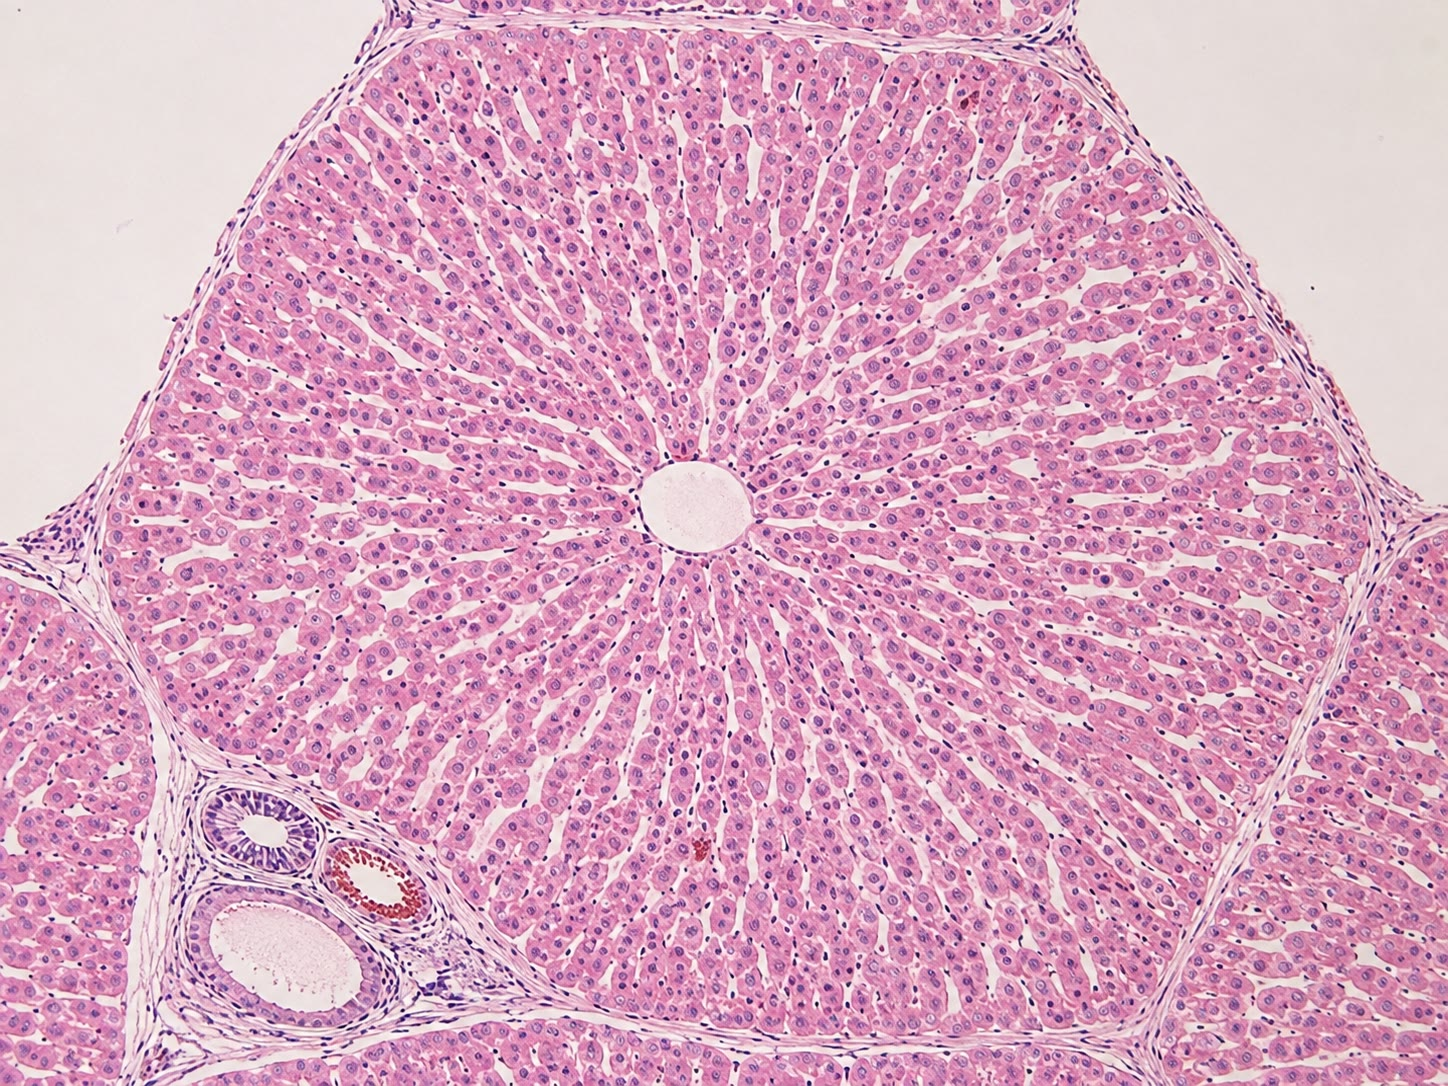
\includegraphics[width=0.52\linewidth]{images/book3/ai/b3-16-liver-lobule-micrograph.jpg}

{\small 肝小叶：肝\omterm{def:b1:cell-unit-of-life:cell}{细胞}板从中央
静脉呈放射状排列，浸于来自肠道的血液中。这些\omterm{def:b1:cell-unit-of-life:cell}{细胞}储存\omterm{def:b1:carbohydrates:polysaccharide}{糖原}，
合成葡萄糖、\omterm{def:b1:lipids:triglyceride}{脂肪}和酮体，并处理含氮废物——是身体的
代谢交换中心。}
\end{omfigure}

\begin{method}[读取代谢状态]\label{met:b1:biosyntheses-integration:state}
\begin{enumerate}
  \item 先看哪种燃料充足：葡萄糖充足则意味着储存
        （先合成\omterm{def:b1:carbohydrates:polysaccharide}{糖原}，再合成\omterm{def:b1:lipids:triglyceride}{脂肪}）；葡萄糖不足则意味着动员。
  \item 追踪信号：胰岛素激活合成酶，抑制磷酸化酶和\omterm{def:b1:lipids:triglyceride}{脂肪}酶；
        胰高血糖素则作用相反，
        ——主要通过对同一批酶进行磷酸化来实现
        （见\cref{ch:b1:enzymes}）。
  \item 检查关键分叉点：\omterm{def:b1:water-small-molecules:atp}{ATP} 与柠檬酸抑制 PFK，并开启\omterm{def:b1:biosyntheses-integration:gluconeogenesis}{糖异生}；
        AMP 作用相反；丙二酰\omterm{def:b1:enzymes:enzyme}{辅酶} A 抑制
        \omterm{def:b1:lipids:triglyceride}{脂肪}分解，此时正在合成\omterm{def:b1:lipids:triglyceride}{脂肪}；乙酰\omterm{def:b1:enzymes:enzyme}{辅酶} A 激活
        启动\omterm{def:b1:biosyntheses-integration:gluconeogenesis}{糖异生}的羧化酶。
  \item 分配\omterm{def:b1:mammal-organization:organ}{器官}任务：肝脏（储存、合成并输出葡萄糖；
        合成酮体和尿素），肌肉（自身储存\omterm{def:b1:carbohydrates:polysaccharide}{糖原}，
        输出乳酸和丙氨酸），\omterm{def:b1:lipids:triglyceride}{脂肪}\omterm{def:b1:body-plans-tissues:tissue}{组织}（储存并释放\omterm{def:b1:lipids:triglyceride}{脂肪}），
        脑（先利用葡萄糖，再利用酮体）。
\end{enumerate}
\end{method}

\section{整合的植物}

\begin{proposition}[源与库]\label{prop:b1:biosyntheses-integration:sourcesink}
白天，叶片的\omterm{def:b1:photosynthesis:chloroplast}{叶绿体}把丙糖磷酸输出到\omterm{def:b1:eukaryotic-cell:organelle}{细胞溶胶}，
在那里合成\emph{蔗糖}，经\omterm{def:b1:flowering-plant-organization:tissues}{韧皮部}运输，
（见\cref{ch:b1:plant-transport}）运往根、果实和生长点；
\omterm{def:b1:flowering-plant-organization:tissues}{韧皮部}运不走的部分则以
\emph{\omterm{def:b1:carbohydrates:polysaccharide}{淀粉}}形式保存在\omterm{def:b1:photosynthesis:chloroplast}{叶绿体}中，作为暂时的储备，夜间动用，以维持蔗糖的持续输出。
哺乳动物的肝脏依据激素决定储存为\omterm{def:b1:carbohydrates:polysaccharide}{糖原}还是输出，
而叶片则依据\omterm{def:b1:eukaryotic-cell:organelle}{细胞溶胶}中的磷酸水平，决定合成\omterm{def:b1:carbohydrates:polysaccharide}{淀粉}还是蔗糖，
这一水平控制着
\omterm{def:b1:photosynthesis:chloroplast}{叶绿体}被膜上的输出转运体。植物依据自身代谢物的浓度调节，
各\omterm{def:b1:mammal-organization:organ}{器官}各自为政；哺乳动物则在此之上
叠加神经与激素的统一指令。
\end{proposition}

\begin{omfigure}
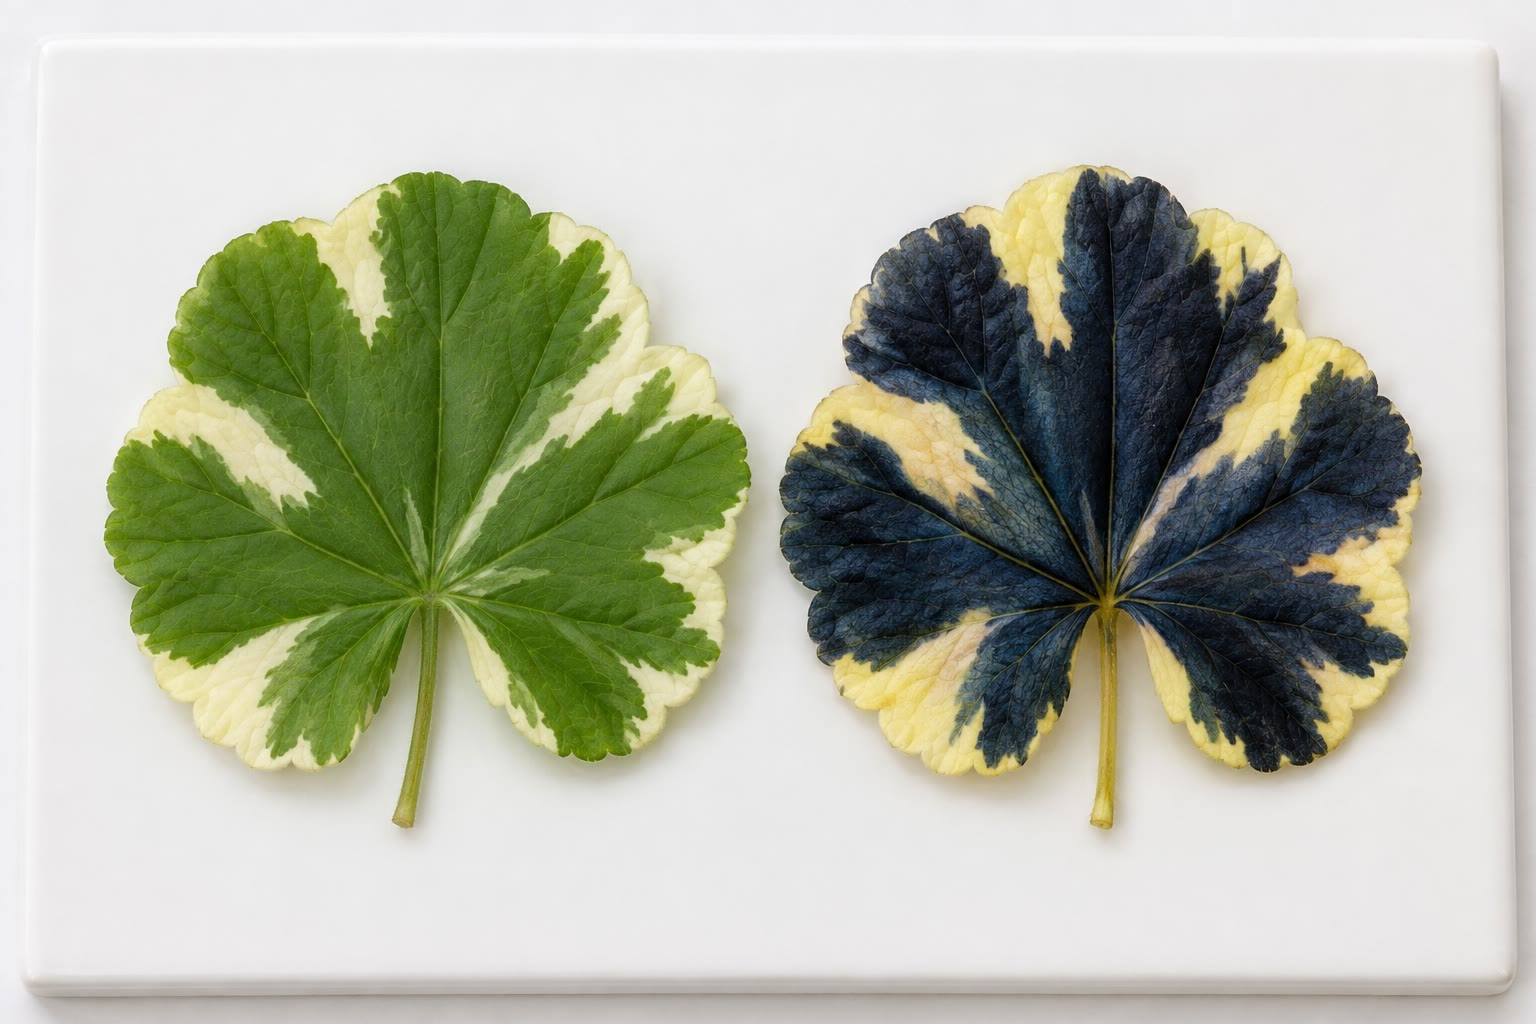
\includegraphics[width=0.6\linewidth]{images/book3/ai/b3-16-variegated-leaf-iodine.jpg}

{\small 斑叶在碘染前后的对比：\omterm{def:b1:carbohydrates:polysaccharide}{淀粉}
（蓝黑色）只出现在含\omterm{def:b1:photosynthesis:pigments}{叶绿素}的部位。白色
区域从绿色部分输入蔗糖，
自身并未合成\omterm{def:b1:carbohydrates:polysaccharide}{淀粉}。}
\end{omfigure}

\begin{example}[一夜的淀粉]\label{ex:b1:biosyntheses-integration:nightstarch}
叶片把白天固定的碳约一半以\omterm{def:b1:carbohydrates:polysaccharide}{淀粉}形式保存，
并在夜间以几乎恒定的速率降解，因此\omterm{def:b1:carbohydrates:polysaccharide}{淀粉}恰好在
黎明前耗尽：人为缩短黑夜，\omterm{def:b1:carbohydrates:polysaccharide}{淀粉}会有剩余；
延长黑夜，植物则在最后几个小时饥饿。
速率在黑暗开始后的第一小时内调整，
依据储存量和预期的夜长确定——
这是由酶和“时钟”完成的一种运算，发生在没有脑的\omterm{def:b1:cell-unit-of-life:cell}{细胞}中。
\end{example}

\section{练习}

\begin{exercise}[$\star$]\label{exo:b1:biosyntheses-integration:1}
写出一个生物合成过程所需的三种物质，以及
为动物\omterm{def:b1:cell-unit-of-life:cell}{细胞}提供大部分 \omterm{def:b1:biosyntheses-integration:ppp}{NADPH} 的途径。
\end{exercise}

\begin{exercise}[$\star$]\label{exo:b1:biosyntheses-integration:2}
列出\omterm{def:b1:respiration-fermentation:glycolysis}{糖酵解}的三个不可逆步骤，以及\omterm{def:b1:biosyntheses-integration:gluconeogenesis}{糖异生}中
绕过每一步的酶。
\end{exercise}

\begin{exercise}[$\star$]\label{exo:b1:biosyntheses-integration:3}
根据血糖图，读出早餐后的峰值、
回落到 \qty{5}{mmol/L} 所需的时间，以及夜间的最低值。
\end{exercise}

\begin{exercise}[$\star$]\label{exo:b1:biosyntheses-integration:4}
为什么发芽的向日葵种子能用油脂制造糖，
而饥饿的人却不能？
\end{exercise}

\begin{exercise}[$\star\star$]\label{exo:b1:biosyntheses-integration:5}
计算由两分子乳酸合成一分子葡萄糖所消耗的 \omterm{def:b1:water-small-molecules:atp}{ATP}，以及
一轮科里循环的净耗能（肌肉获得 2，肝脏消耗 6）。
由谁付出，付出什么？
\end{exercise}

\begin{exercise}[$\star\star$]\label{exo:b1:biosyntheses-integration:6}
合成一分子棕榈酸需要 8 个乙酰\omterm{def:b1:enzymes:enzyme}{辅酶} A、7 个 \omterm{def:b1:water-small-molecules:atp}{ATP} 和 14 个 \omterm{def:b1:biosyntheses-integration:ppp}{NADPH}。需要多少个葡萄糖分子
经\omterm{def:b1:respiration-fermentation:glycolysis}{糖酵解}和丙酮酸脱氢酶反应，才能提供乙酰\omterm{def:b1:enzymes:enzyme}{辅酶} A，
又需要多少个葡萄糖分子经\omterm{def:b1:biosyntheses-integration:ppp}{戊糖磷酸途径}
（每个葡萄糖产生 2 个 \omterm{def:b1:biosyntheses-integration:ppp}{NADPH}）才能提供 \omterm{def:b1:biosyntheses-integration:ppp}{NADPH}？
\end{exercise}

\begin{exercise}[$\star\star$]\label{exo:b1:biosyntheses-integration:7}
解释\omterm{def:b1:biosyntheses-integration:fasynthesis}{脂肪酸合成}与 $\beta$-氧化为何使用不同的
酶、不同的区室和不同的\omterm{def:b1:enzymes:enzyme}{辅酶}，以及
丙二酰\omterm{def:b1:enzymes:enzyme}{辅酶} A 如何阻止二者同时进行。
\end{exercise}

\begin{exercise}[$\star\star$]\label{exo:b1:biosyntheses-integration:8}
写出丙氨酸与 $\alpha$-酮戊二酸的转氨反应，
并命名其产物。进食\omterm{def:b1:proteins:peptide}{蛋白质}后哪个方向的反应占优，
禁食时又是哪个方向？
\end{exercise}

\begin{exercise}[$\star\star$]\label{exo:b1:biosyntheses-integration:9}
某患者缺乏葡萄糖-6-磷酸酶。预测其两餐之间的血糖、
肝脏大小以及血乳酸的变化，
并说明理由。
\end{exercise}

\begin{exercise}[$\star\star\star$]\label{exo:b1:biosyntheses-integration:10}
大脑每天需要 \qty{120}{g} 葡萄糖，\qty{1}{g} \omterm{def:b1:proteins:peptide}{蛋白质}
可生成 \qty{0.55}{g} 葡萄糖。计算禁食者仅靠\omterm{def:b1:biosyntheses-integration:gluconeogenesis}{糖异生}为大脑供能时每天损失的\omterm{def:b1:proteins:peptide}{蛋白质}量，
并换算为所代表的肌肉量
（\omterm{def:b1:proteins:peptide}{蛋白质}含量为 \qty{20}{\%}）。若酮体使大脑的葡萄糖需求降至 \qty{40}{g}，
试说明酮体带来了哪些变化。
\end{exercise}

\begin{exercise}[$\star\star\star$]\label{exo:b1:biosyntheses-integration:11}
胰岛素激活\omterm{def:b1:carbohydrates:polysaccharide}{糖原}合酶，使\omterm{def:b1:carbohydrates:polysaccharide}{糖原}磷酸化酶失活，
胰高血糖素则作用相反。解释二者为何不能同时活跃，
若同时活跃会发生什么（计算每个循环浪费的 \omterm{def:b1:water-small-molecules:atp}{ATP}：
添加一个葡萄糖需消耗一个 UTP，移除则不耗能），以及
这一“无效循环”在熊蜂为飞行肌升温中
有何作用。
\end{exercise}

\begin{exercise}[$\star\star\star$]\label{exo:b1:biosyntheses-integration:12}
“\omterm{def:b1:cell-unit-of-life:cell}{细胞}没有蓝图，只有阀门。”请用一段话讨论：
交汇点酶的别构调控与激素调控，
催化相反方向反应的独立酶所起的作用，
以及由此涌现出的、看似蓝图的规律。
\end{exercise}

\section{问题：人的二十四小时}

\begin{problem}[{周末问题——不吃早餐的一天：称量储备
、供给大脑、计算蛋白质并动员脂肪，
最后算出肝糖原可维持的
禁食时长}]
\label{pb:b1:biosyntheses-integration:1}
一位体重 \qty{70}{kg} 的成年人每天消耗 \qty{8.4}{MJ}（
平均功率 \qty{100}{W}），体内储存有：肝\omterm{def:b1:carbohydrates:polysaccharide}{糖原} \qty{100}{g}，肌\omterm{def:b1:carbohydrates:polysaccharide}{糖原}
\qty{400}{g}，\omterm{def:b1:lipids:triglyceride}{脂肪} \qty{12}{kg}，\omterm{def:b1:proteins:peptide}{蛋白质} \qty{10}{kg}（其中
\qty{6}{kg} 位于肌肉中）。大脑每天消耗 \qty{120}{g} 葡萄糖，
（\qty{5}{g/h}）；其他依赖葡萄糖的\omterm{def:b1:body-plans-tissues:tissue}{组织}（红\omterm{def:b1:cell-unit-of-life:cell}{细胞}、肾髓质）
消耗 \qty{40}{g}。能量值：碳水化合物 \qty{17}{kJ/g}，\omterm{def:b1:lipids:triglyceride}{脂肪}
\qty{38}{kJ/g}，\omterm{def:b1:proteins:peptide}{蛋白质} \qty{17}{kJ/g}；\qty{1}{g} \omterm{def:b1:proteins:peptide}{蛋白质}经
\omterm{def:b1:biosyntheses-integration:gluconeogenesis}{糖异生}可生成 \qty{0.55}{g} 葡萄糖；\qty{1}{g} \omterm{def:b1:lipids:triglyceride}{脂肪}可
（通过其甘油）生成 \qty{0.1}{g} 葡萄糖。

\medskip
\noindent\textbf{第一部分——储备。}
\begin{enumerate}
  \item 计算四种储备中各自所含的能量，以
        兆焦计，以及每种储备可维持的消耗天数。
  \item 哪一种储备可直接向血液供应葡萄糖？为何
        肌\omterm{def:b1:carbohydrates:polysaccharide}{糖原}不能？
  \item 计算身体每天为依赖葡萄糖的\omterm{def:b1:body-plans-tissues:tissue}{组织}
        所需的葡萄糖总量。
  \item 计算血液本身所含的葡萄糖（\qty{5}{mmol/L}，
        \qty{5}{L}、\qty{180}{g/mol}），以及它单独
        可供大脑使用多少分钟。
  \item 大脑所用葡萄糖占每日消耗的比例是多少？
  \item 进餐后，肝\omterm{def:b1:carbohydrates:polysaccharide}{糖原}已充满，而血糖仍在
        上升。请说出葡萄糖的下一去向，以及
        决定这一去向的激素。
\end{enumerate}

\medskip
\noindent\textbf{第二部分——夜晚。}
末次进餐于 20:00 结束；此后血液中的葡萄糖
完全由肝脏供应。
\begin{enumerate}[resume]
  \item 若依赖葡萄糖的\omterm{def:b1:body-plans-tissues:tissue}{组织}每天需要 \qty{160}{g} 葡萄糖，
        则其每小时的需求量是多少？
  \item \qty{100}{g} 肝\omterm{def:b1:carbohydrates:polysaccharide}{糖原}按此速率可维持多久，
        若除此之外无其他来源供应葡萄糖？
  \item 事实上，\omterm{def:b1:biosyntheses-integration:gluconeogenesis}{糖异生}在最初几小时内提供约三分之一的
        葡萄糖。请重新计算肝\omterm{def:b1:carbohydrates:polysaccharide}{糖原}的持续时间。
  \item 肝\omterm{def:b1:carbohydrates:polysaccharide}{糖原}在早晨几点耗尽？请按每种估算
        分别给出结果。
  \item 与此同时，肌肉消耗\omterm{def:b1:lipids:fattyacid}{脂肪酸}。计算夜间
        （\qty{12}{h}）被氧化的\omterm{def:b1:lipids:triglyceride}{脂肪}量，已知其
        占静息消耗的 \qty{60}{\%}，且仅燃烧\omterm{def:b1:lipids:triglyceride}{脂肪}。
\end{enumerate}

\medskip
\noindent\textbf{第三部分——次日，不进食。}
\begin{enumerate}[resume]
  \item \omterm{def:b1:carbohydrates:polysaccharide}{糖原}耗尽后，\qty{160}{g}葡萄糖必须
        来自\omterm{def:b1:biosyntheses-integration:gluconeogenesis}{糖异生}。计算每天所需的\omterm{def:b1:proteins:peptide}{蛋白质}量，以及
        它所对应的肌肉质量。
  \item 计算肝脏由丙酮酸生成\qty{160}{g}葡萄糖
        所消耗的 \omterm{def:b1:water-small-molecules:atp}{ATP}（每个葡萄糖消耗 6 个 \omterm{def:b1:water-small-molecules:atp}{ATP}），
        以及在\qty{50}{kJ/mol}下的能量。
  \item 计算\omterm{def:b1:lipids:triglyceride}{脂肪}中甘油的贡献：若\omterm{def:b1:lipids:triglyceride}{脂肪}承担全部非葡萄糖能量消耗，
        每天需氧化多少\omterm{def:b1:lipids:triglyceride}{脂肪}，
        其甘油可生成多少葡萄糖？
  \item 重新计算所需\omterm{def:b1:proteins:peptide}{蛋白质}量，
        并扣除甘油的贡献。
  \item 按此速率，多少天后一半肌肉会消失？
  \item 从第三天起，肝脏生成酮体，
        大脑由酮体提供三分之二的能量；
        葡萄糖需求降至大脑 \qty{40}{g}、其余部分 \qty{40}{g}。
        重新计算每天的\omterm{def:b1:proteins:peptide}{蛋白质}损失，
        以及失去一半肌肉所需的天数。
  \item 计算\omterm{def:b1:lipids:triglyceride}{脂肪}储备在每天 \qty{8.4}{MJ} 下可维持的天数，
        （长期禁食时降至 \qty{6.5}{MJ}，请重新计算）。
  \item 解释禁食者为何在\omterm{def:b1:lipids:triglyceride}{脂肪}耗尽之前因\omterm{def:b1:proteins:peptide}{蛋白质}损失而死亡，
        以及酮体所延缓的过程。
\end{enumerate}

\medskip
\noindent\textbf{第四部分——调控开关。}
\begin{enumerate}[resume]
  \item 写出肝脏中在 03:00 必须活跃的酶，
        在 09:00 必须失活的酶，
        以及\omterm{def:b1:carbohydrates:polysaccharide}{糖原}代谢中作用相反的酶。
  \item 写出分别设定两种状态的信号（激素），
        以及其发挥作用所经由的化学修饰。
  \item 03:00 时，肝\omterm{def:b1:cell-unit-of-life:cell}{细胞}因\omterm{def:b1:lipids:triglyceride}{脂肪}氧化而含有大量乙酰\omterm{def:b1:enzymes:enzyme}{辅酶} A。
        写出由此被激活的\omterm{def:b1:biosyntheses-integration:gluconeogenesis}{糖异生}酶，
        以及同时被 \omterm{def:b1:water-small-molecules:atp}{ATP} 抑制的\omterm{def:b1:respiration-fermentation:glycolysis}{糖酵解}酶。
  \item 解释\omterm{def:b1:biosyntheses-integration:gluconeogenesis}{糖异生}与\omterm{def:b1:respiration-fermentation:glycolysis}{糖酵解}若在同一\omterm{def:b1:cell-unit-of-life:cell}{细胞}中同时进行，
        则只会把 \omterm{def:b1:water-small-molecules:atp}{ATP} 转化为热量，
        并说明三处旁路上各自独立的酶如何避免这一情况。
  \item 无胰岛素的糖尿病患者血糖很高，但肝脏仍持续生成葡萄糖和酮体。
        试从这些调控开关出发，
        解释这一矛盾。
  \item 陈述结果：肝脏\omterm{def:b1:carbohydrates:polysaccharide}{糖原}可维持的禁食小时数
        （分别包括和不包括\omterm{def:b1:biosyntheses-integration:gluconeogenesis}{糖异生}两种情况），
        转为酮体前后每天的\omterm{def:b1:proteins:peptide}{蛋白质}损失，
        以及\omterm{def:b1:lipids:triglyceride}{脂肪}储备可维持的天数。
\end{enumerate}
\end{problem}
